
\section{Method}
Suppose we are given a paired motion--text dataset $\mathcal{D}=\{(m^{(j)}, t^{(j)})\}_{j=1}^{N}$.
For simplicity, we omit the sample index $(j)$ when there is no ambiguity.
Each sample consists of a motion sequence $m \in \mathbb{R}^{T_m' \times D_m}$ and a text sequence $t \in \mathbb{R}^{T_t' \times D_t}$. Our goal is to learn fine-grained motion--text alignment.
We model the alignment between a motion sequence and a text sequence as an optimal transport plan
$\mathbf{P}$,
where each entry $P_{uv}$ measures the semantic correspondence between the $u$-th motion frame and the $v$-th text token. We define the transport plan in \cref{sec:ot} and then provide an intuitive analysis of this formulation in \cref{sec:case}. Finally, we describe the feature extraction process in \cref{sec:network} and the CLIP-style contrastive training objective in \cref{sec:training}.

\subsection{Optimal Transport Cost}
\label{sec:ot}
Our model consists of a motion feature extractor $E_m$ and a text feature extractor $E_t$.
Given a motion sequence $m$ and a text sequence $t$, $E_m$ produces a sequence of fine-grained motion features
\begin{equation}
Z^m=\{z^m_1,\ldots,z^m_{T_m}\},
\end{equation}
and $E_t$ produces a sequence of text features
\begin{equation}
Z^t=\{z^t_1,\ldots,z^t_{T_t}\}.
\end{equation}
Note that $T_m\neq T_m'$ and $T_t\neq T_t'$ due to down-sampling in the encoders. Let $s(\cdot,\cdot)$ denote the cosine similarity between $\ell_2$-normalized features.

We define the transport cost matrix $\mathbf{C}\in\mathbb{R}^{T_m\times T_t}$ by
\begin{equation}
\label{eq:cost_matrix}
\mathbf{C}_{uv}=1-s(z^m_u,z^t_v).
\end{equation}
Intuitively, a smaller cost indicates a stronger semantic correspondence between the $u$-th motion frame and the $v$-th text token.

Based on the admissible transport set $U(\mathbf{a},\mathbf{b})$ defined in the previous subsection, we define the OT cost for a motion--text pair $(m,t)$ as
\begin{equation}
\label{eq:ot_single}
\mathcal{J}_{\mathrm{OT}}(m,t)
=
\min_{\mathbf{P}\in U(\mathbf{a},\mathbf{b})}
\langle \mathbf{P},\mathbf{C}\rangle.
\end{equation}

This OT cost measures the minimum transport cost required to align the motion and text features under the marginal constraints.
A lower value of $\mathcal{J}_{\mathrm{OT}}(m,t)$ indicates better fine-grained motion--text alignment. As in \cref{sec:entro}, we follow \cref{eq:entropic_ot} to obtain approximated optimal transport plan $\mathbf{P}'$. The estimated optimal transport cost is 
\begin{equation}
\label{eq:eot}
\mathcal{J}_{\mathrm{EOT}} = \langle \mathbf{P}',\mathbf{C}\rangle
\end{equation}
Although $\mathbf{P}'$ is a function of $\mathbf{C}$, we treat it as a constant during backpropagation for simplicity. Under this approximation, $\mathcal{J}_{\mathrm{EOT}}$ remains differentiable with respect to $\mathbf{C}$.


\subsection{Analysis: a Case Study}
\label{sec:case}
To better understand how the proposed objective encourages fine-grained alignment, we consider an idealized case in which each motion frame is described by exactly one text token.

\begin{assumption}[Perfect Frame--Token Correspondence]
\label{asmp:perfect_alignment}
Assume that the motion and text sequences have equal lengths, i.e., $T_m=T_t$.
Further assume that there exist encoder parameters $\theta_m$ and $\theta_t$ such that, for each paired sample $(m,t)$, there exists a bijection
$\pi:\{1,\ldots,T_m\}\rightarrow\{1,\ldots,T_t\}$ satisfying
\begin{equation}
s\!\left(z^m_u,z^t_{\pi(u)}\right)=1,
\quad \forall u\in\{1,\ldots,T_m\},
\end{equation}
where $z^m_u$ and $z^t_v$ denote the $u$-th and $v$-th output features of $E_m(m;\theta_m)$ and $E_t(t;\theta_t)$, respectively.
\end{assumption}

\begin{theorem}[Zero OT Cost under Perfect Alignment]
\label{thm:zero_ot}
Under Assumption~\ref{asmp:perfect_alignment}, the OT objective $\mathcal{J}_{OT}(m,t)$ admits a feasible transport plan with zero cost. Specifically, the transport plan defined by
\begin{equation}
P_{uv}=\frac{1}{T_m}\mathbbm{1}\{v=\pi(u)\}
\end{equation}
is feasible and achieves
\begin{equation}
\mathcal{J}_{OT}(m,t)=0.
\end{equation}
\end{theorem}

\begin{proof} See supplementary.
\end{proof}

In practice, motion-text alignment is generally many-to-many rather than bijective. Nevertheless, \cref{thm:zero_ot} shows that the proposed objective is consistent with perfect fine-grained alignment in an idealized setting, which helps explain why minimizing $\mathcal{J}_{\mathrm{OT}}$ can encourage meaningful motion--text correspondence in practice.

\begin{algorithm}
\caption{CLIP-style Motion--Text Training with Sinkhorn-based Alignment}
\label{alg:ot_motion_text}
\begin{algorithmic}[1]
\REQUIRE Paired dataset $\mathcal{D}=\{(m^{(j)},t^{(j)})\}_{j=1}^N$;
motion feature extractor $E_m(\cdot;\theta_m)$; text feature extractor $E_t(\cdot;\theta_t)$
\ENSURE Trained parameters $\theta_m,\theta_t$

\FOR{each training epoch}
    \FOR{each mini-batch $\{(m^{(i)},t^{(i)})\}_{i=1}^B$}
        \FOR{$i=1$ to $B$}
            \STATE $Z^{m,(i)} \leftarrow E_m(m^{(i)};\theta_m)$
            \STATE $Z^{t,(i)} \leftarrow E_t(t^{(i)};\theta_t)$
            \STATE $\ell_2$-normalize all feature vectors in $Z^{m,(i)}$ and $Z^{t,(i)}$
        \ENDFOR

        \FOR{$i=1$ to $B$}
            \FOR{$j=1$ to $B$}
                \STATE \textcolor{green!50!black}{Construct the cost matrix $\mathbf{C}^{(i,j)}$ from $Z^{m,(i)}$ and $Z^{t,(j)}$ according to \cref{eq:cost_matrix}}
                \STATE \textcolor{green!50!black}{Compute the Sinkhorn transport plan $P^{(i,j)} \in U(\mathbf{a},\mathbf{b})$ according to \cref{eq:entropic_ot}.} 
                \STATE \textcolor{green!50!black}{Compute the pairwise alignment logit $L_{ij} = -\mathcal{J}_{\mathrm{EOT}}(m^{(i)}, t^{(j)})$ using \cref{eq:ot_single}}
            \ENDFOR
        \ENDFOR

        \STATE Compute motion-to-text probabilities $p(t^{(j)}\mid m^{(i)})$ by row-wise softmax over $L$
        \STATE Compute text-to-motion probabilities $p(m^{(i)}\mid t^{(j)})$ by column-wise softmax over $L$
        \STATE Compute the symmetric contrastive loss $\mathcal{L}=\frac{1}{2}(\mathcal{L}_{m2t}+\mathcal{L}_{t2m})$
        \STATE Update $\theta_m,\theta_t$ by minimizing $\mathcal{L}$
    \ENDFOR
\ENDFOR
\end{algorithmic}
\end{algorithm}

\begin{figure*}
    \centering
    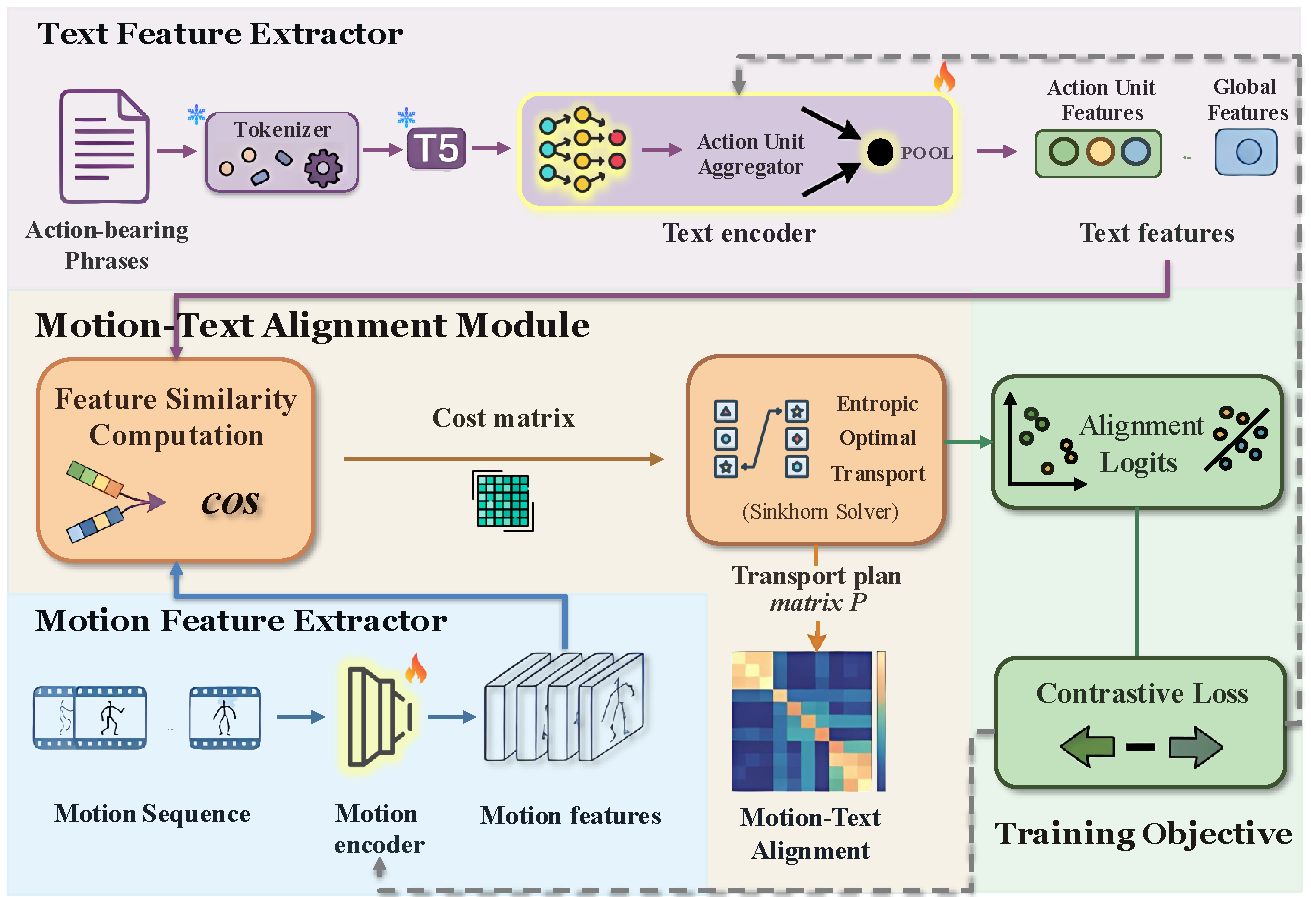
\includegraphics[width=0.95\linewidth]{author-kit-CVPR2026-v1-latex-/figs/pipeline.pdf}
    \caption{Overview of \ours. The text stream first encodes the action-bearing phrases with a frozen T5 backbone. Then the action unit aggregator aggregates the features into action unit features and the global feature, which form a text feature set. In parallel, the motion stream extracts temporal motion features using a temporal-convolution-based encoder. Given the motion and text features, we compute a feature-similarity-based cost matrix and solve an entropic optimal transport problem with the Sinkhorn algorithm to obtain pairwise alignment logits. These logits are then used in a CLIP-style symmetric contrastive objective for training.}
    \label{fig:pipeline}
\end{figure*}

\subsection{Feature Extraction}
\label{sec:network}
The semi-supervised learning framework is illustrated in \cref{fig:pipeline}. Our architecture adopts a dual-stream design to learn representations from textual descriptions and motion sequences. The original expressive text annotation is first segmented into multiple \textbf{action-bearing phrases} using an LLM (details are in the supplementary material). These phrases are then concatenated into a sequence and fed into the text feature extractor. The text feature extractor $E_t$ leverages a frozen T5-base~\cite{2020t5} backbone to extract latent semantic features, which are subsequently projected into a latent space through an additional MLP. To facilitate temporal alignment, we introduce an \textbf{action unit aggregator} that groups tokens belonging to the same phrase and pools their embeddings into compact \textbf{action unit features}. Some motion segments may not be explicitly described by any action-bearing phrase in the text. To avoid imposing spurious correspondences, we do not force every motion frame to align with an action-unit representation alone and allow a motion frame to correspond to an \texttt{[UNK]} token. We introduce a \textbf{global feature} mechanism that aggregates sequence-level information and provides holistic semantic context for the contrastive objective. This global feature is appended to the action unit features to form the \textbf{text features} $Z^t$ in \cref{alg:ot_motion_text}. On the motion stream $E_m$, we finetune the pre-trained VQ-VAE encoder~\cite{guo2025snapmogen}, composed of temporal convolutional layers, to extract \textbf{motion features} $Z^m$ from motion sequences.

\subsection{Training Objective}
\label{sec:training}
As illustrated in \cref{alg:ot_motion_text}, the training process is conceptually similar to CLIP~\cite{radford2021learning}, in that both methods learn cross-modal representations through batch-wise contrastive supervision over paired motion--text samples. We highlight in green the steps that differ from standard CLIP training.

Given a mini-batch of paired samples
$\mathcal{D}$,
CLIP first computes a global representation for each sample in the two modalities and then forms a batch-wise similarity matrix, where the diagonal entries correspond to matched pairs and the off-diagonal entries correspond to mismatched pairs. A symmetric cross-entropy objective is subsequently applied to encourage high similarity for ground-truth pairs and low similarity for mismatched pairs.

Our training pipeline follows the same high-level paradigm, but differs in how the pairwise alignment score is computed. Instead of directly measuring similarity between two global embeddings, we first compute a fine-grained motion--text alignment cost using the entropy-regularized OT objective in \cref{eq:entropic_ot}. Specifically, for each pair $(m^{(i)}, t^{(j)})$ in the batch, we compute
\begin{equation}
\label{eq:pairwise_eot}
L_{ij} = -\mathcal{J}_{\mathrm{EOT}}(m^{(i)}, t^{(j)}),
\end{equation}
where a larger $L_{ij}$ indicates stronger cross-modal alignment.

Using these pairwise alignment logits, we define the motion-to-text matching probability as
\begin{equation}
p(t^{(j)} \mid m^{(i)})
=
\frac{\exp(L_{ij}/\tau)}
{\sum_{k=1}^{B}\exp(L_{ik}/\tau)},
\end{equation}
and analogously define the text-to-motion matching probability as
\begin{equation}
p(m^{(i)} \mid t^{(j)})
=
\frac{\exp(L_{ij}/\tau)}
{\sum_{k=1}^{B}\exp(L_{kj}/\tau)},
\end{equation}
where $\tau$ is a temperature parameter and $B$ is the batch size.

We then optimize the model using a symmetric contrastive loss:
\begin{equation}
\mathcal{L}_{m2t}
=
-\frac{1}{B}\sum_{i=1}^{B}
\log p(t^{(i)} \mid m^{(i)}),
\end{equation}
\begin{equation}
\mathcal{L}_{t2m}
=
-\frac{1}{B}\sum_{i=1}^{B}
\log p(m^{(i)} \mid t^{(i)}),
\end{equation}
and the final training objective is
\begin{equation}
\label{eq:final_training_loss}
\mathcal{L}
=
\frac{1}{2}\left(\mathcal{L}_{m2t}+\mathcal{L}_{t2m}\right).
\end{equation}

Compared with CLIP, the key difference is that our pairwise logits are not produced by a single global embedding similarity. Instead, they are derived from a fine-grained Sinkhorn-based transport cost between motion frames and text units, allowing the model to capture local temporal correspondence while still benefiting from batch-wise contrastive supervision.




